%!TEX root = book.tex

\chapter{Giới thiệu}
\label{cha:introduce}



Những năm gần đây, AI - Artificial Intelligence (Trí Tuệ Nhân Tạo), và cụ thể hơn là Machine Learning (Học Máy hoặc Máy Học - {\it Với những từ chuyên ngành, tôi sẽ dùng song song cả tiếng Anh và tiếng Việt, tuy nhiên sẽ ưu tiên tiếng Anh vì thuận tiện hơn trong việc tra cứu}) nổi lên như một bằng chứng của cuộc cách mạng công nghiệp lần thứ tư (1 - động cơ hơi nước, 2 - năng lượng điện, 3 - công nghệ thông tin). Trí Tuệ Nhân Tạo đang len lỏi vào mọi lĩnh vực trong đời sống mà có thể chúng ta không nhận ra. Xe tự hành của Google và Tesla, hệ thống tự tag khuôn mặt trong ảnh của Facebook, trợ lý ảo Siri của Apple, hệ thống gợi ý sản phẩm của Amazon, hệ thống gợi ý phim của Netflix, máy chơi cờ vây AlphaGo của Google DeepMind, ..., chỉ là một vài trong vô vàn những ứng dụng của AI/Machine Learning. (Xem thêm \href{{https://www.facebook.com/zuck/posts/10103351073024591}}{Jarvis - trợ lý thông minh cho căn nhà của Mark Zuckerberg}.)

% \url{https://www.facebook.com/zuck/posts/10103351073024591}


Machine Learning là một tập con của AI. Theo định nghĩa của Wikipedia, {\it Machine learning is the subfield of computer science that "gives computers the ability to learn without being explicitly programmed"}. Nói đơn giản, Machine Learning là một lĩnh vực nhỏ của Khoa Học Máy Tính, nó có khả năng tự học hỏi dựa trên dữ liệu đưa vào mà không cần phải được lập trình cụ thể. Bạn Nguyễn Xuân Khánh tại đại học Maryland đang viết một cuốn sách về Machine Learning bằng tiếng Việt khá thú vị, các bạn có thể tham khảo bài \href{https://ml-book-vn.khanhxnguyen.com/intro.html}{Machine Learning là gì?}.

Những năm gần đây, {khi mà khả năng tính toán} của các máy tính được nâng lên một tầm cao mới và lượng dữ liệu khổng lồ được thu thập bởi các hãng công nghệ lớn, Machine Learning đã tiến thêm một bước tiến dài và một lĩnh vực mới được ra đời gọi là Deep Learning (Học Sâu). Deep Learning đã giúp máy tính thực thi những việc tưởng chừng như không thể vào 10 năm trước: phân loại cả ngàn vật thể khác nhau trong các bức ảnh, tự tạo chú thích cho ảnh, bắt chước giọng nói và chữ viết của con người, giao tiếp với con người, hay thậm chí cả sáng tác văn hay âm nhạc (Xem thêm \href{{http://machinelearningmastery.com/inspirational-applications-deep-learning/}}{8 Inspirational Applications of Deep Learning}).

Mối quan hệ giữa Artificial Intelligence, Machine Learning, và Deep Learning được cho trong Hình \ref{fig:aimldl}.

\begin{figure}
\centering
	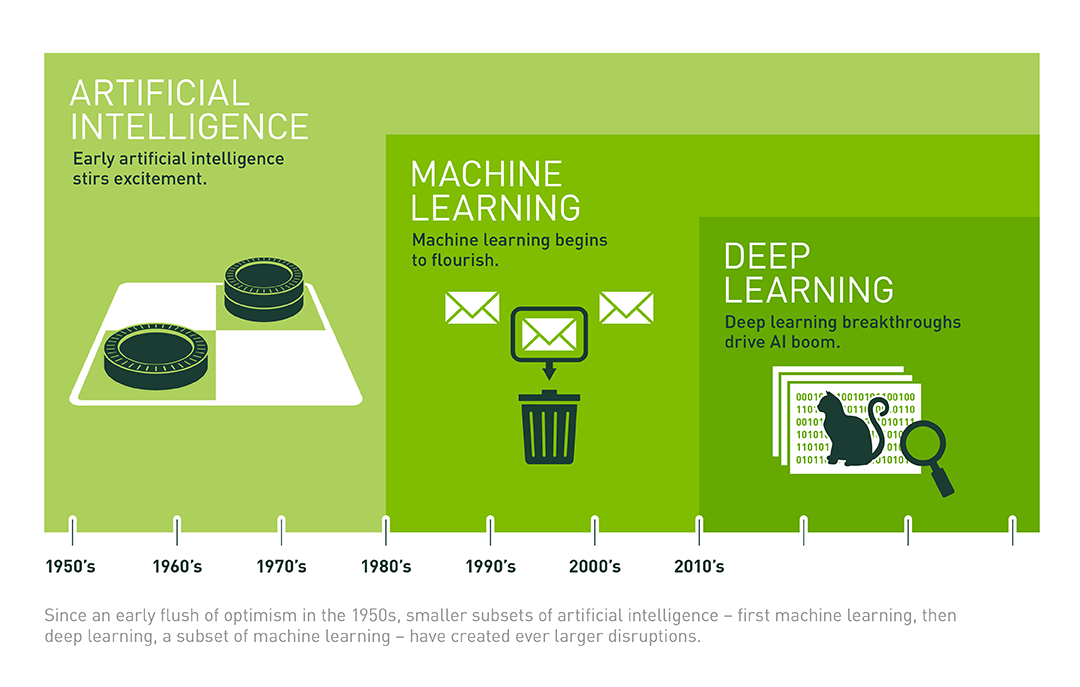
\includegraphics[width = \textwidth]{../introduce/aimldl.png}
	\caption[]{Mối quan hệ giữa AI, Machine Learning và Deep Learning. Nguồn: \href{https://blogs.nvidia.com/blog/2016/07/29/whats-difference-artificial-intelligence-machine-learning-deep-learning-ai/}{What’s the Difference Between Artificial Intelligence, Machine Learning, and Deep Learning?}}
	\label{fig:aimldl}
\end{figure}

% <div class="imgcap">
% <div >
%     <img src="/assets/introduce/aimldl.png" width = "800"></a>
%     <!-- <img src="/assets/rl/mdp.png" height="206"> -->
% </div>
% <div class="thecap">Mối quan hệ giữa AI, Machine Learning và Deep Learning. <br> (Nguồn: <a href="https://blogs.nvidia.com/blog/2016/07/29/whats-difference-artificial-intelligence-machine-learning-deep-learning-ai/">What’s the Difference Between Artificial Intelligence, Machine Learning, and Deep Learning?</a>)</div>
% </div>

\section{Mục đích viết Blog}
Nhu cầu về nhân lực ngành Machine Learning (Deep Learning) đang ngày một cao, kéo theo đó nhu cầu học Machine Learning trên thế giới và ở Việt Nam ngày một lớn. Cá nhân tôi cũng muốn hệ thống lại kiến thức của mình về lĩnh vực này để chuẩn bị cho tương lai (đây là một trong những mục tiêu của tôi trong năm 2017). Tôi sẽ cố gắng đi từ những thuật toán cơ bản nhất của Machine Learning kèm theo các ví dụ và mã nguồn trong mỗi bài viết. Tôi sẽ viết 1-2 tuần 1 bài (việc viết các công thức toán và code trên blog thực sự tốn nhiều thời gian hơn tôi từng nghĩ). Đồng thơi, tôi cũng mong muốn nhận được phản hồi của bạn đọc để qua những thảo luận, tôi và các bạn có thể nắm bắt được các thuật toán này. 

Khi chuẩn bị các bài viết, tôi sẽ giả định rằng bạn đọc có một chút kiến thức về Đại Số Tuyến Tính (Linear Algebra), Xác Suât Thống Kê (Probability and Statistics) và có kinh nghiệm về lập trình Python. Nếu bạn chưa có nhiều kinh nghiệm về các lĩnh vực này, đừng quá lo lắng vì mỗi bài sẽ chỉ sử dụng một vài kỹ thuật cơ bản. Hãy để lại câu hỏi của bạn ở phần Comment bên dưới mỗi bài, tôi sẽ thảo luận thêm với các bạn.

Trong bài tiếp theo của blog này, tôi sẽ giới thiệu về các nhóm thuật toán Machine learning cơ bản. Mời các bạn theo dõi. 

\section{Tham khảo thêm}
\subsection{Các khóa học}
\subsubsection{Tiếng Anh}
\begin{enumerate}
	\item \href{https://www.coursera.org/learn/machine-learning}{Machine Learning với thầy Andrew Ng trên Coursera} ({\it Khóa học nổi tiếng nhất về Machine Learning })

	\item \href{https://www.udacity.com/course/deep-learning--ud730}{Deep Learning by Google trên Udacity} ({\it Khóa học nâng cao hơn về Deep Learning với Tensorflow})


	\item \href{http://machinelearningmastery.com/}{Machine Learning mastery} ({\it Các thuật toán Machine Learning cơ bản})
\end{enumerate}

\subsubsection{Tiếng Việt}
{\bf Lưu ý}: {\it Các khóa học này tôi chưa từng tham gia, chỉ đưa ra để các bạn tham khảo.}
\begin{enumerate}
	\item \href{http://tuanvannguyen.blogspot.com/2016/12/cap-nhat-khoa-hoc-ve-machine-learning.html}{Machine Learning 1/2017}


	\item \href{https://techmaster.vn/khoa-hoc/25511/machine-learning-co-ban}{Nhập môn Machine Learning, Tech Master- Cao Thanh Hà {\it POSTECH}}() 

\end{enumerate}

\subsection{Các trang Machine Learning tiếng Việt khác}
\begin{enumerate}
	\item \href{http://viet.jnlp.org/kien-thuc-co-ban-ve-xu-ly-ngon-ngu-tu-nhien/machine-learning-trong-nlp}{Machine Learning trong Xử Lý Ngôn Ngữ Tự Nhiên - Nhóm Đông Du {\it Nhật Bản}}

	\item \href{https://ongxuanhong.wordpress.com/}{Machine Learning cho người mới bắt đầu - Ông Xuân Hồng {\it JAIST}}. 

	
	 \item \href{https://ml-book-vn.khanhxnguyen.com/}{Machine Learning book for Vietnamese - Nguyễn Xuân Khánh \textit{University of Maryland}}
\end{enumerate}
% 3. [Machine Learning trong Xử Lý Ngôn Ngữ Tự Nhiên - Nhóm Đông Du _Nhật Bản_](http://viet.jnlp.org/kien-thuc-co-ban-ve-xu-ly-ngon-ngu-tu-nhien/machine-learning-trong-nlp)
% 4. [Machine Learning cho người mới bắt đầu - Ông Xuân Hồng _JAIST_](https://ongxuanhong.wordpress.com/). 
% 5. [Machine Learning book for Vietnamese - Nguyễn Xuân Khánh _University of Maryland_](https://ml-book-vn.khanhxnguyen.com/)